\appendix
\pagenumbering{Roman}
\thispagestyle{empty}  
\renewcommand{\appendixname}{Appendix}%%přílohy, číslování římskými


\chapter*{Appendix}
\addcontentsline{toc}{chapter}{Appendix}

\section{Technické detaily}

The device comunicates with brltty with the UOBP driver found at \footnote{\url{https://github.com/timthelion/UOBP}}.  The arduino is to be flashed with the FCHAD firmware found at the same url.  The arduino is connected to 8 paralel solenoid circuites as described here \footnote{\url{http://playground.arduino.cc/uploads/Learning/solenoid_driver.pdf}}, using MOSFETs of type IRF530N.  The solenoid power circute is powered by a 6 volt 4 amp wall power supply of type "Smart Electronic Switching adapter Model:JGS1002-24060-2E".  Touches were detected using a 16 channel MUX of type CMOS4067 connected to 4 digital IO pins and one analog pin.  The analog pin was connected to ground with a 10k ohm resistor of type RM0207 "resistor with metalic layer 1\% TK50 0.5W RM 7.5mm".


\clearpage
\begin{figure}
\section{Obrazky FCHADu}
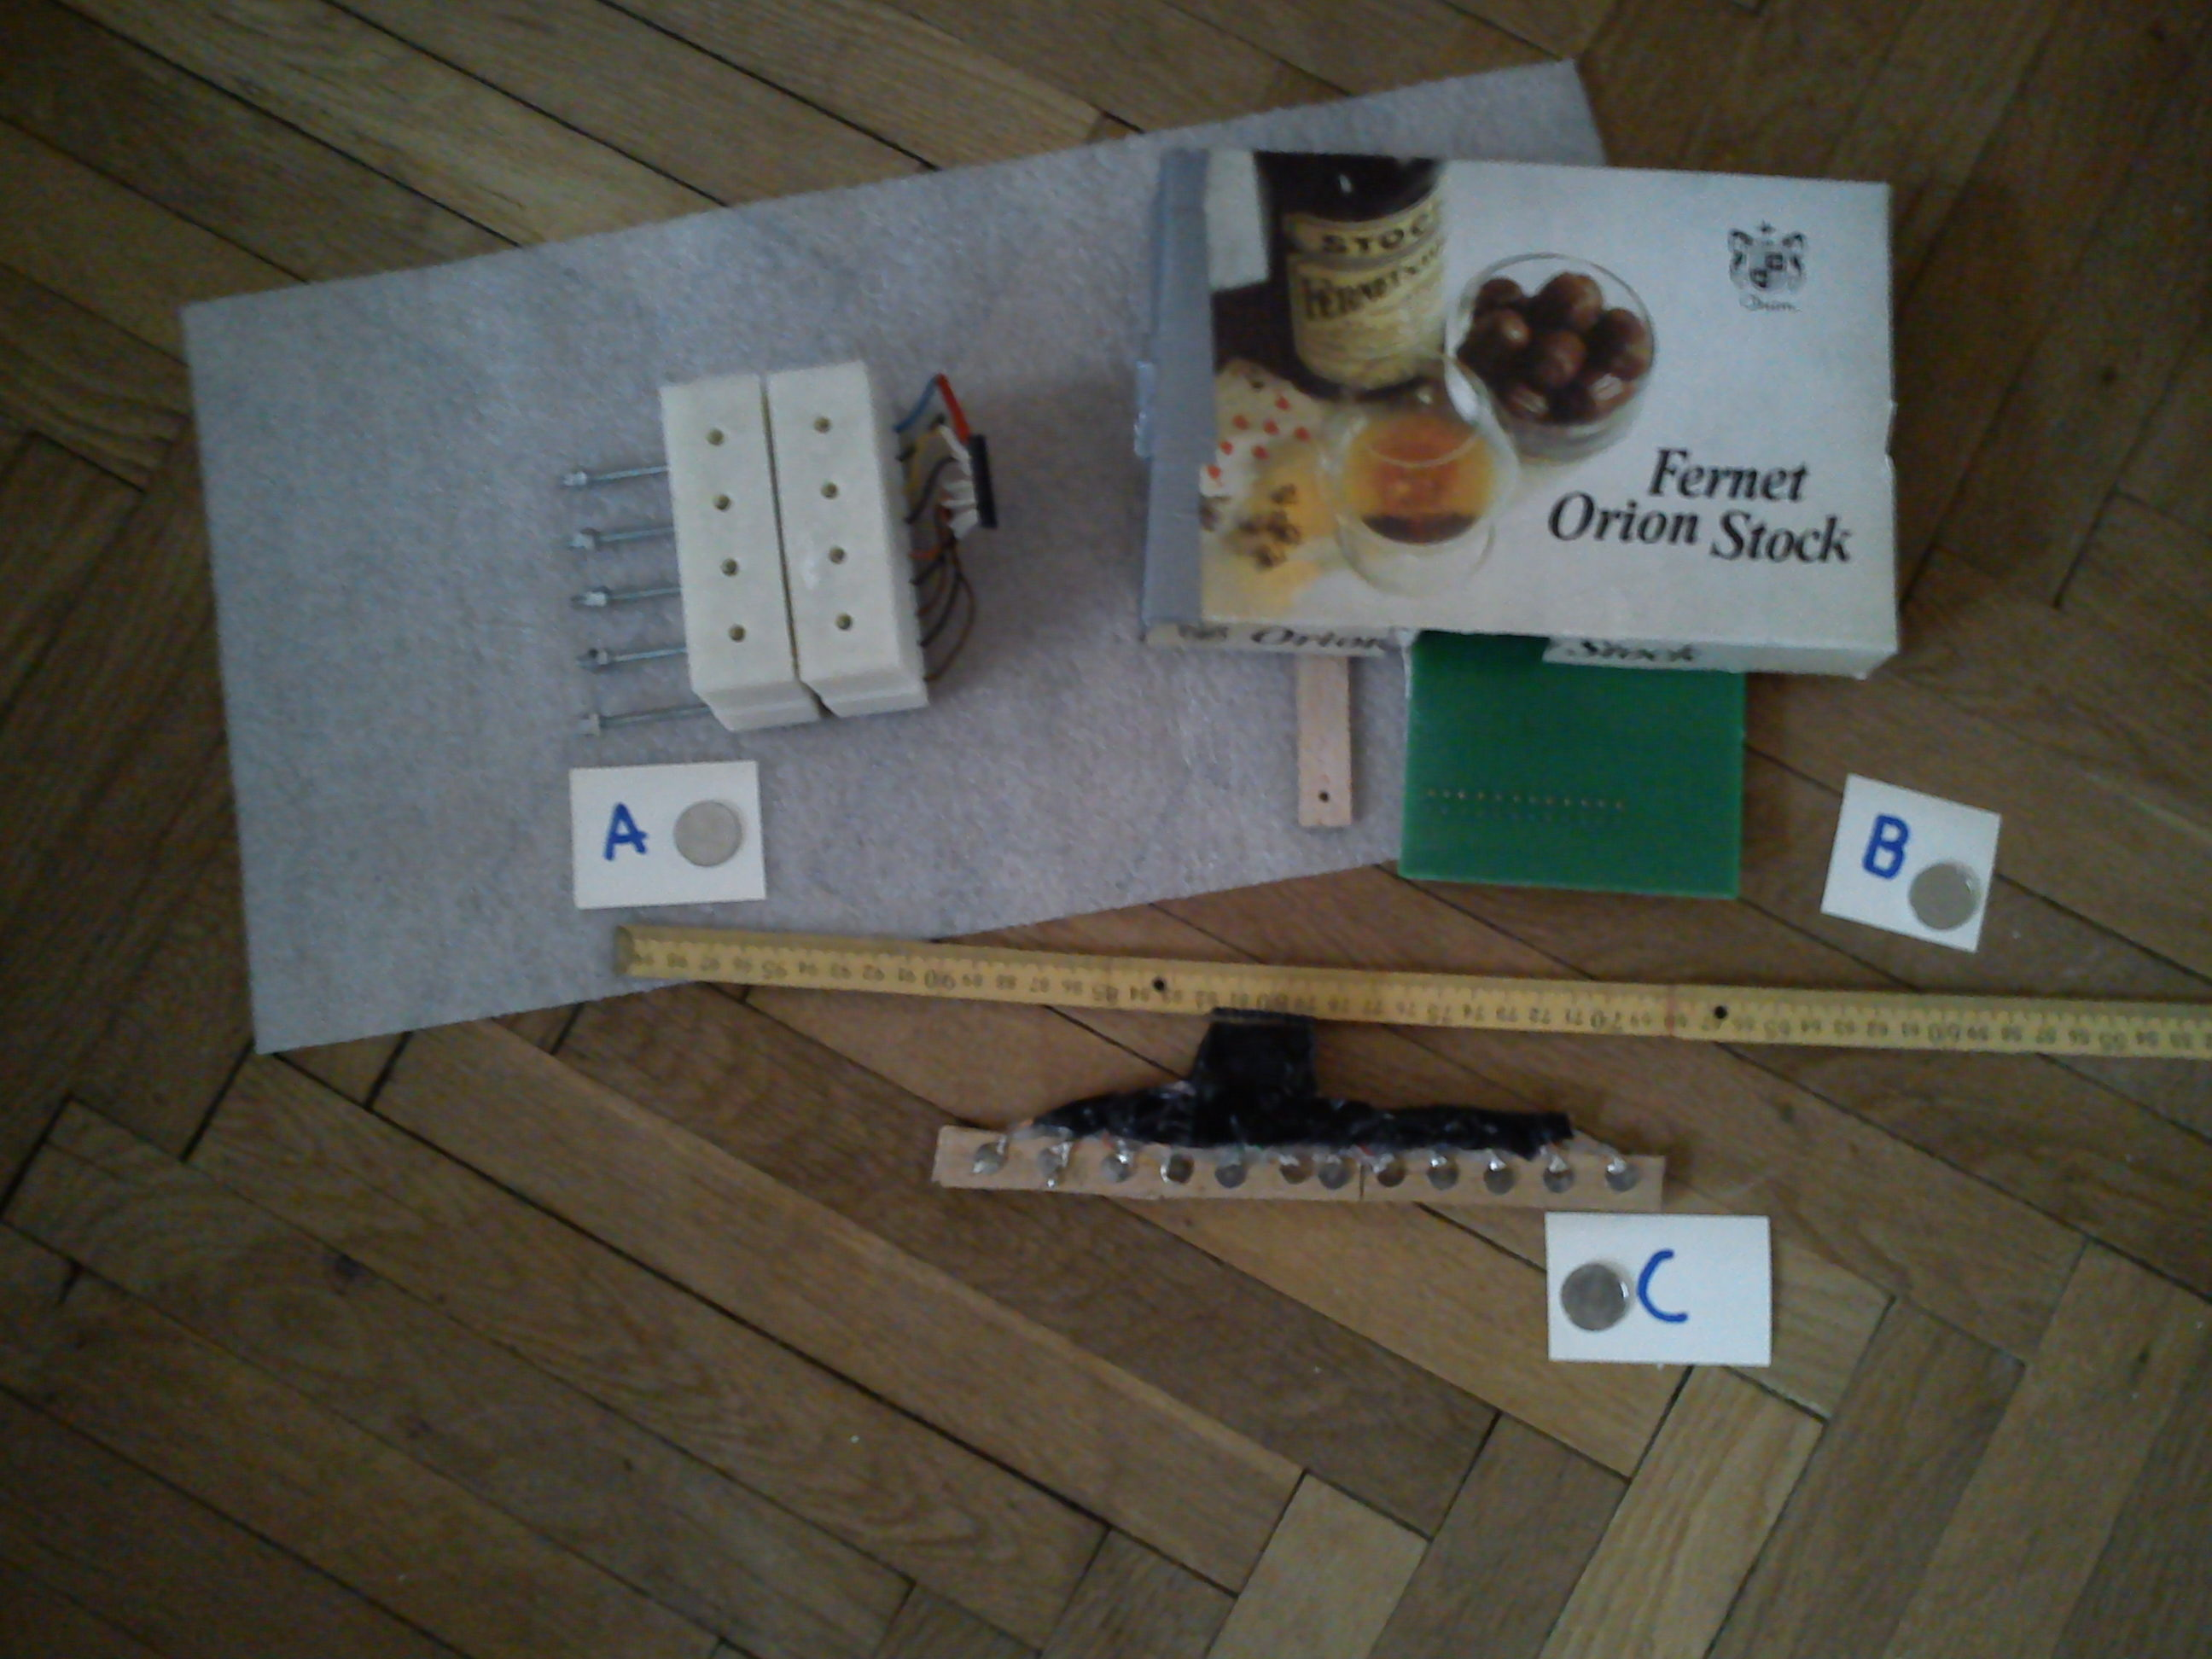
\includegraphics[width=1\textwidth]{Device1}
\begin{subfigure}{.5\textwidth}
  \centering
  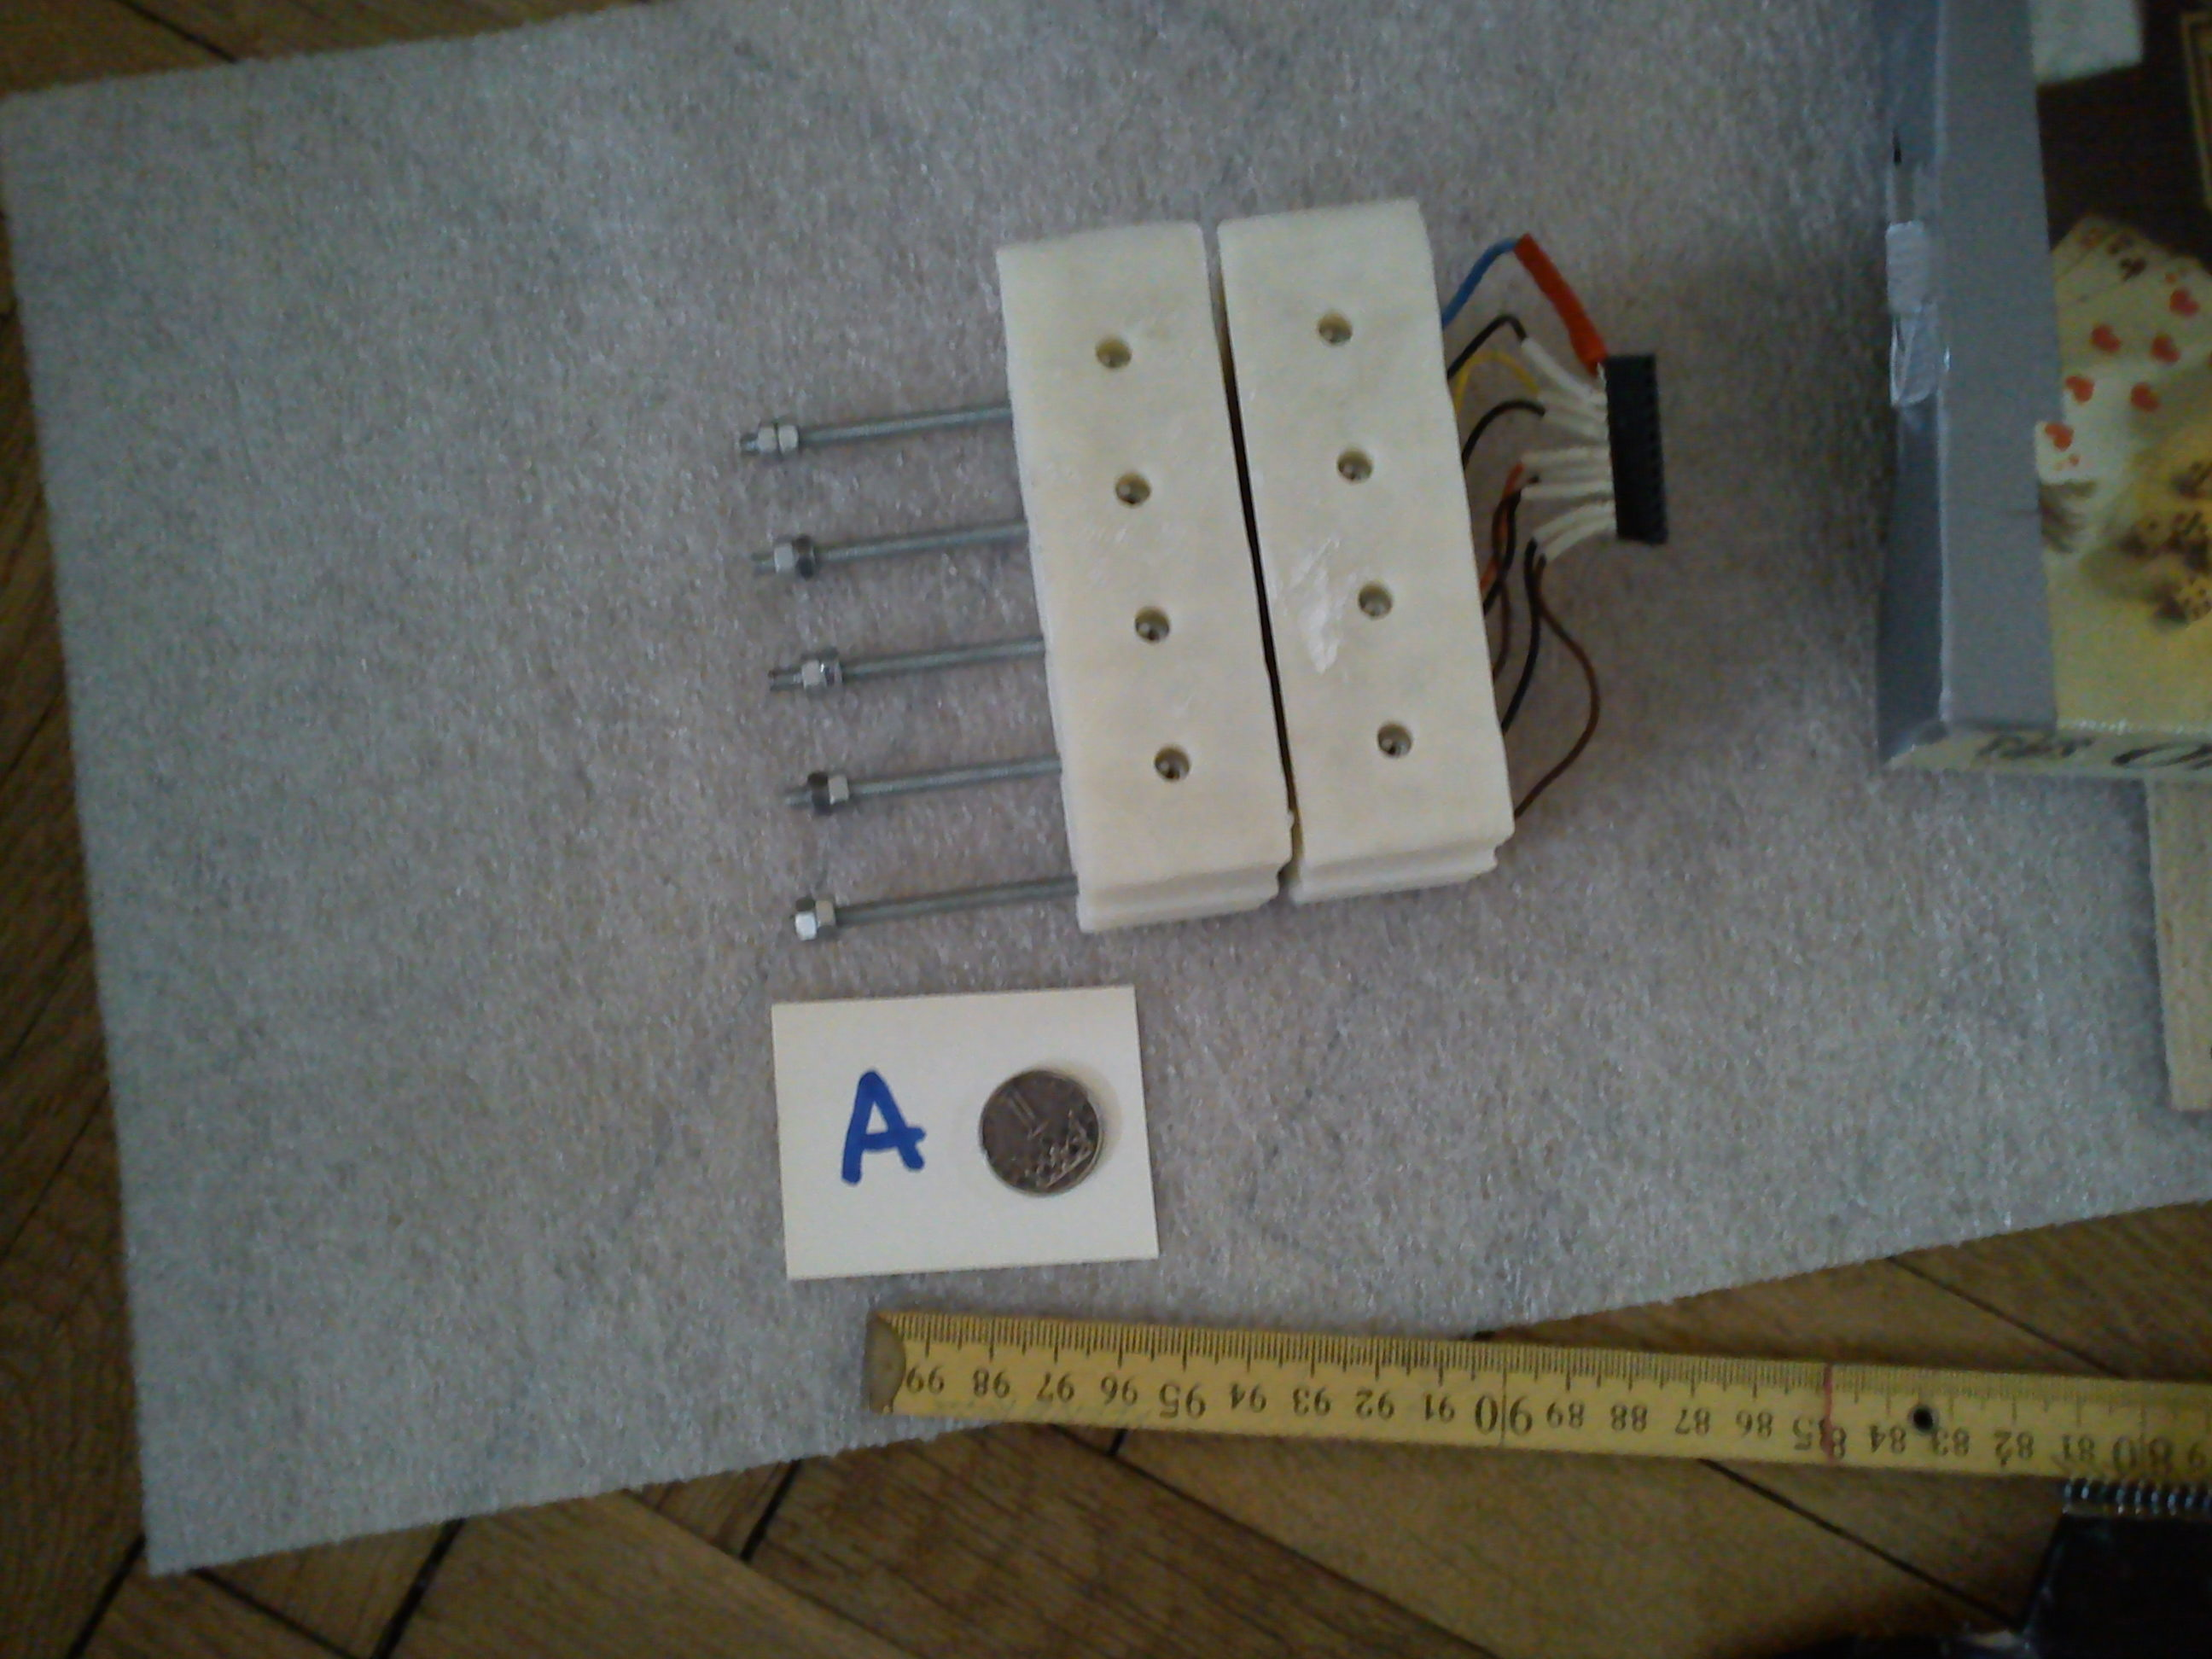
\includegraphics[width=.95\linewidth]{Device1-A}
  \caption{Obrazek 1-A - Zobrazovač}
  \label{fig:sub1}
\end{subfigure}%
\begin{subfigure}{.5\textwidth}
  \centering
  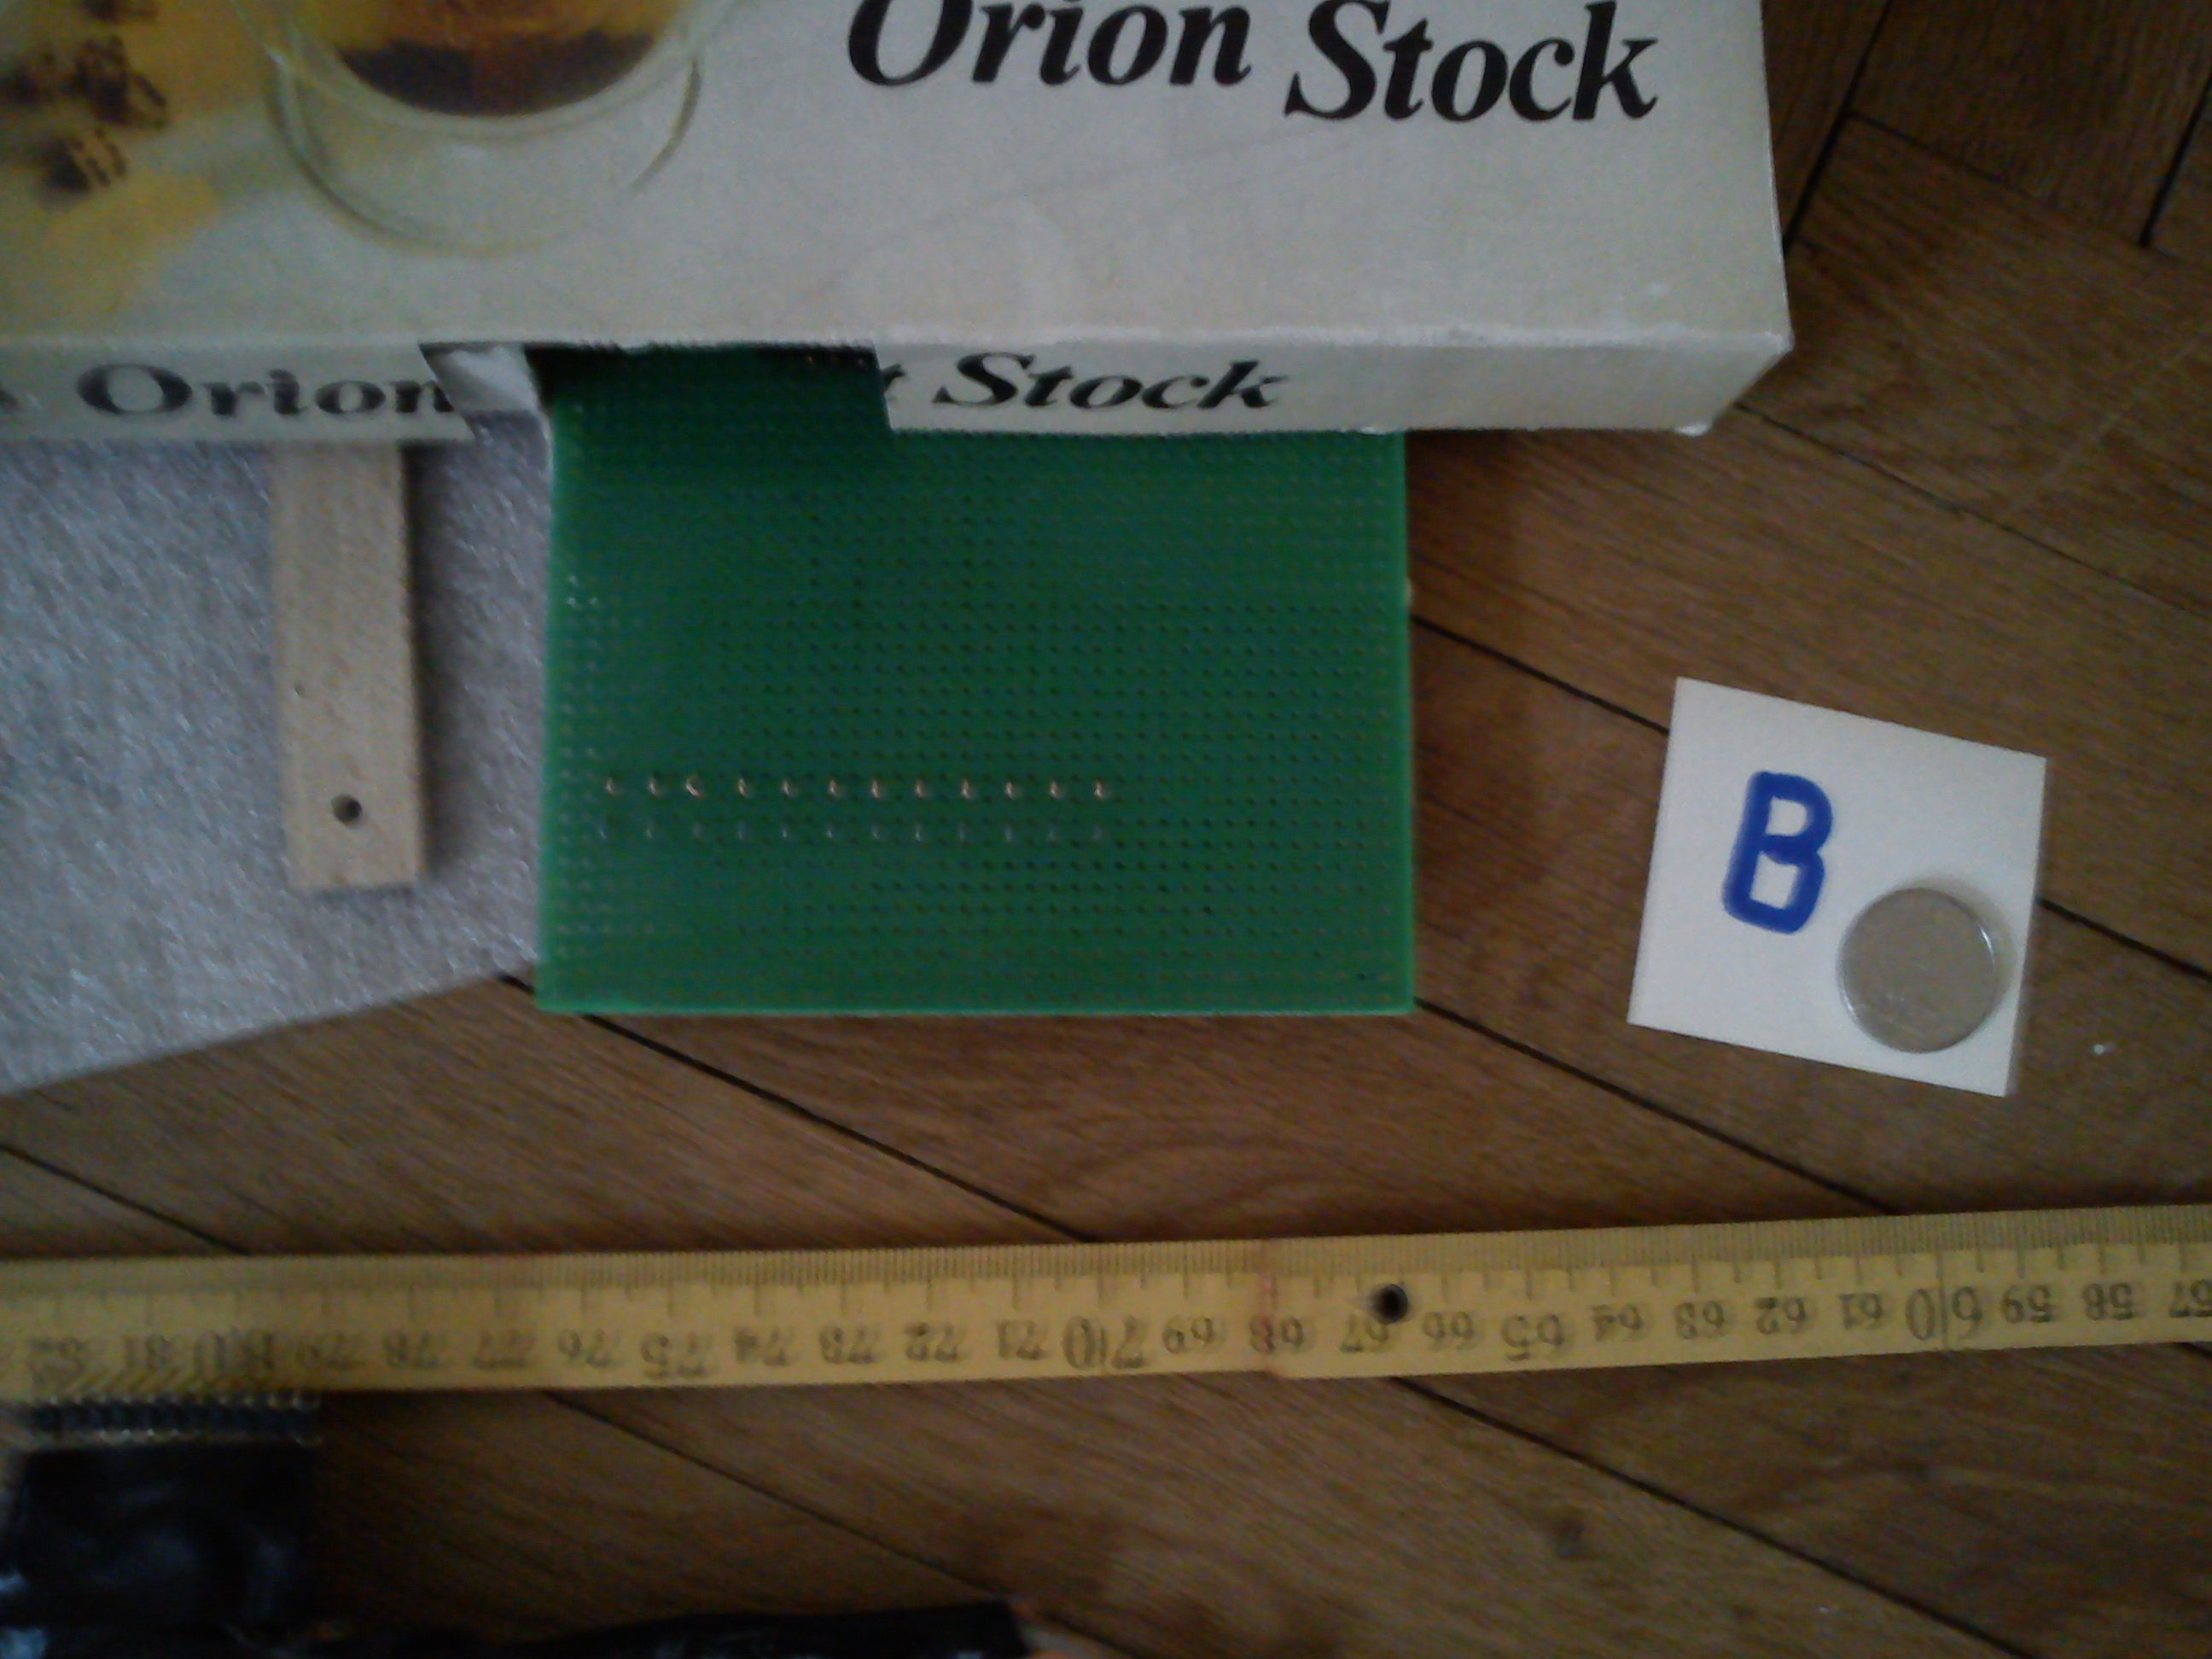
\includegraphics[width=.95\linewidth]{Device1-B}
  \caption{Obrazek 1-B - Kursor selektor}
  \label{fig:sub2}
\end{subfigure}

\label{fig:test}
\end{figure}
\begin{figure}
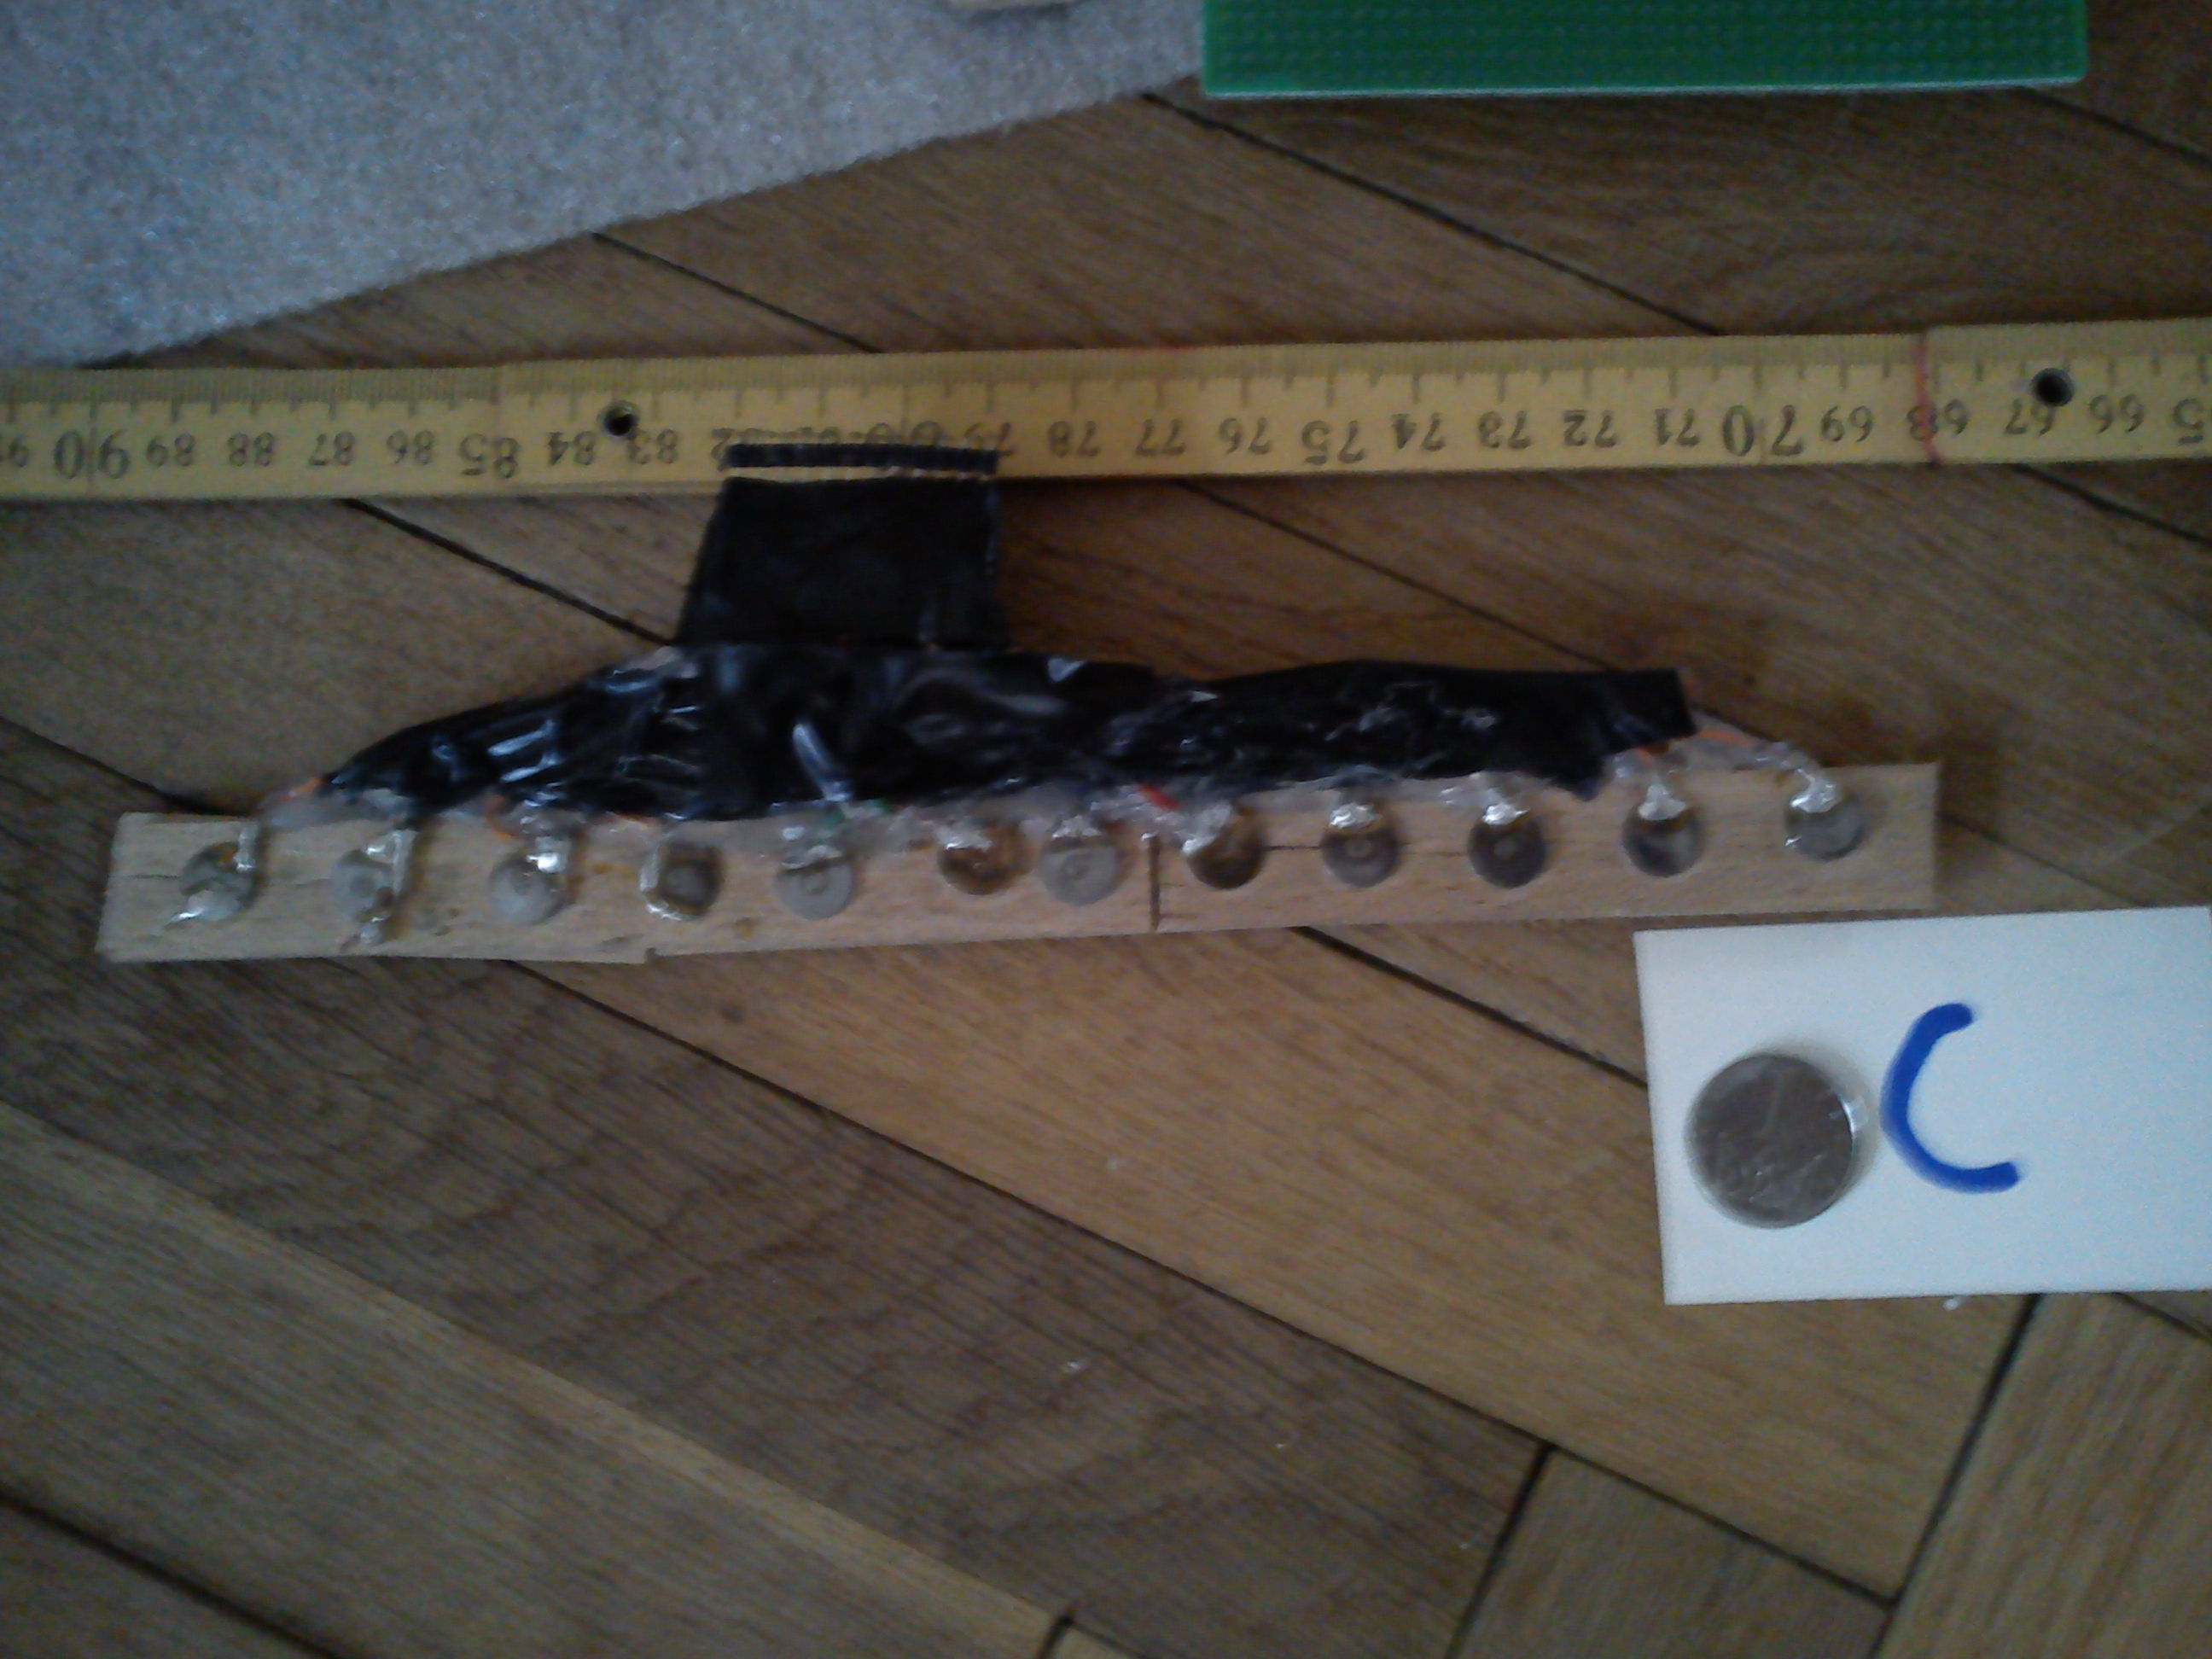
\includegraphics[width=.7\linewidth]{Device1-C}
\caption{Obrazek 1-C - Starý kursor selektor}
\label{fig:sub2}
\end{figure}

\begin{figure}
\centering
\begin{subfigure}{.5\textwidth}
  \centering
  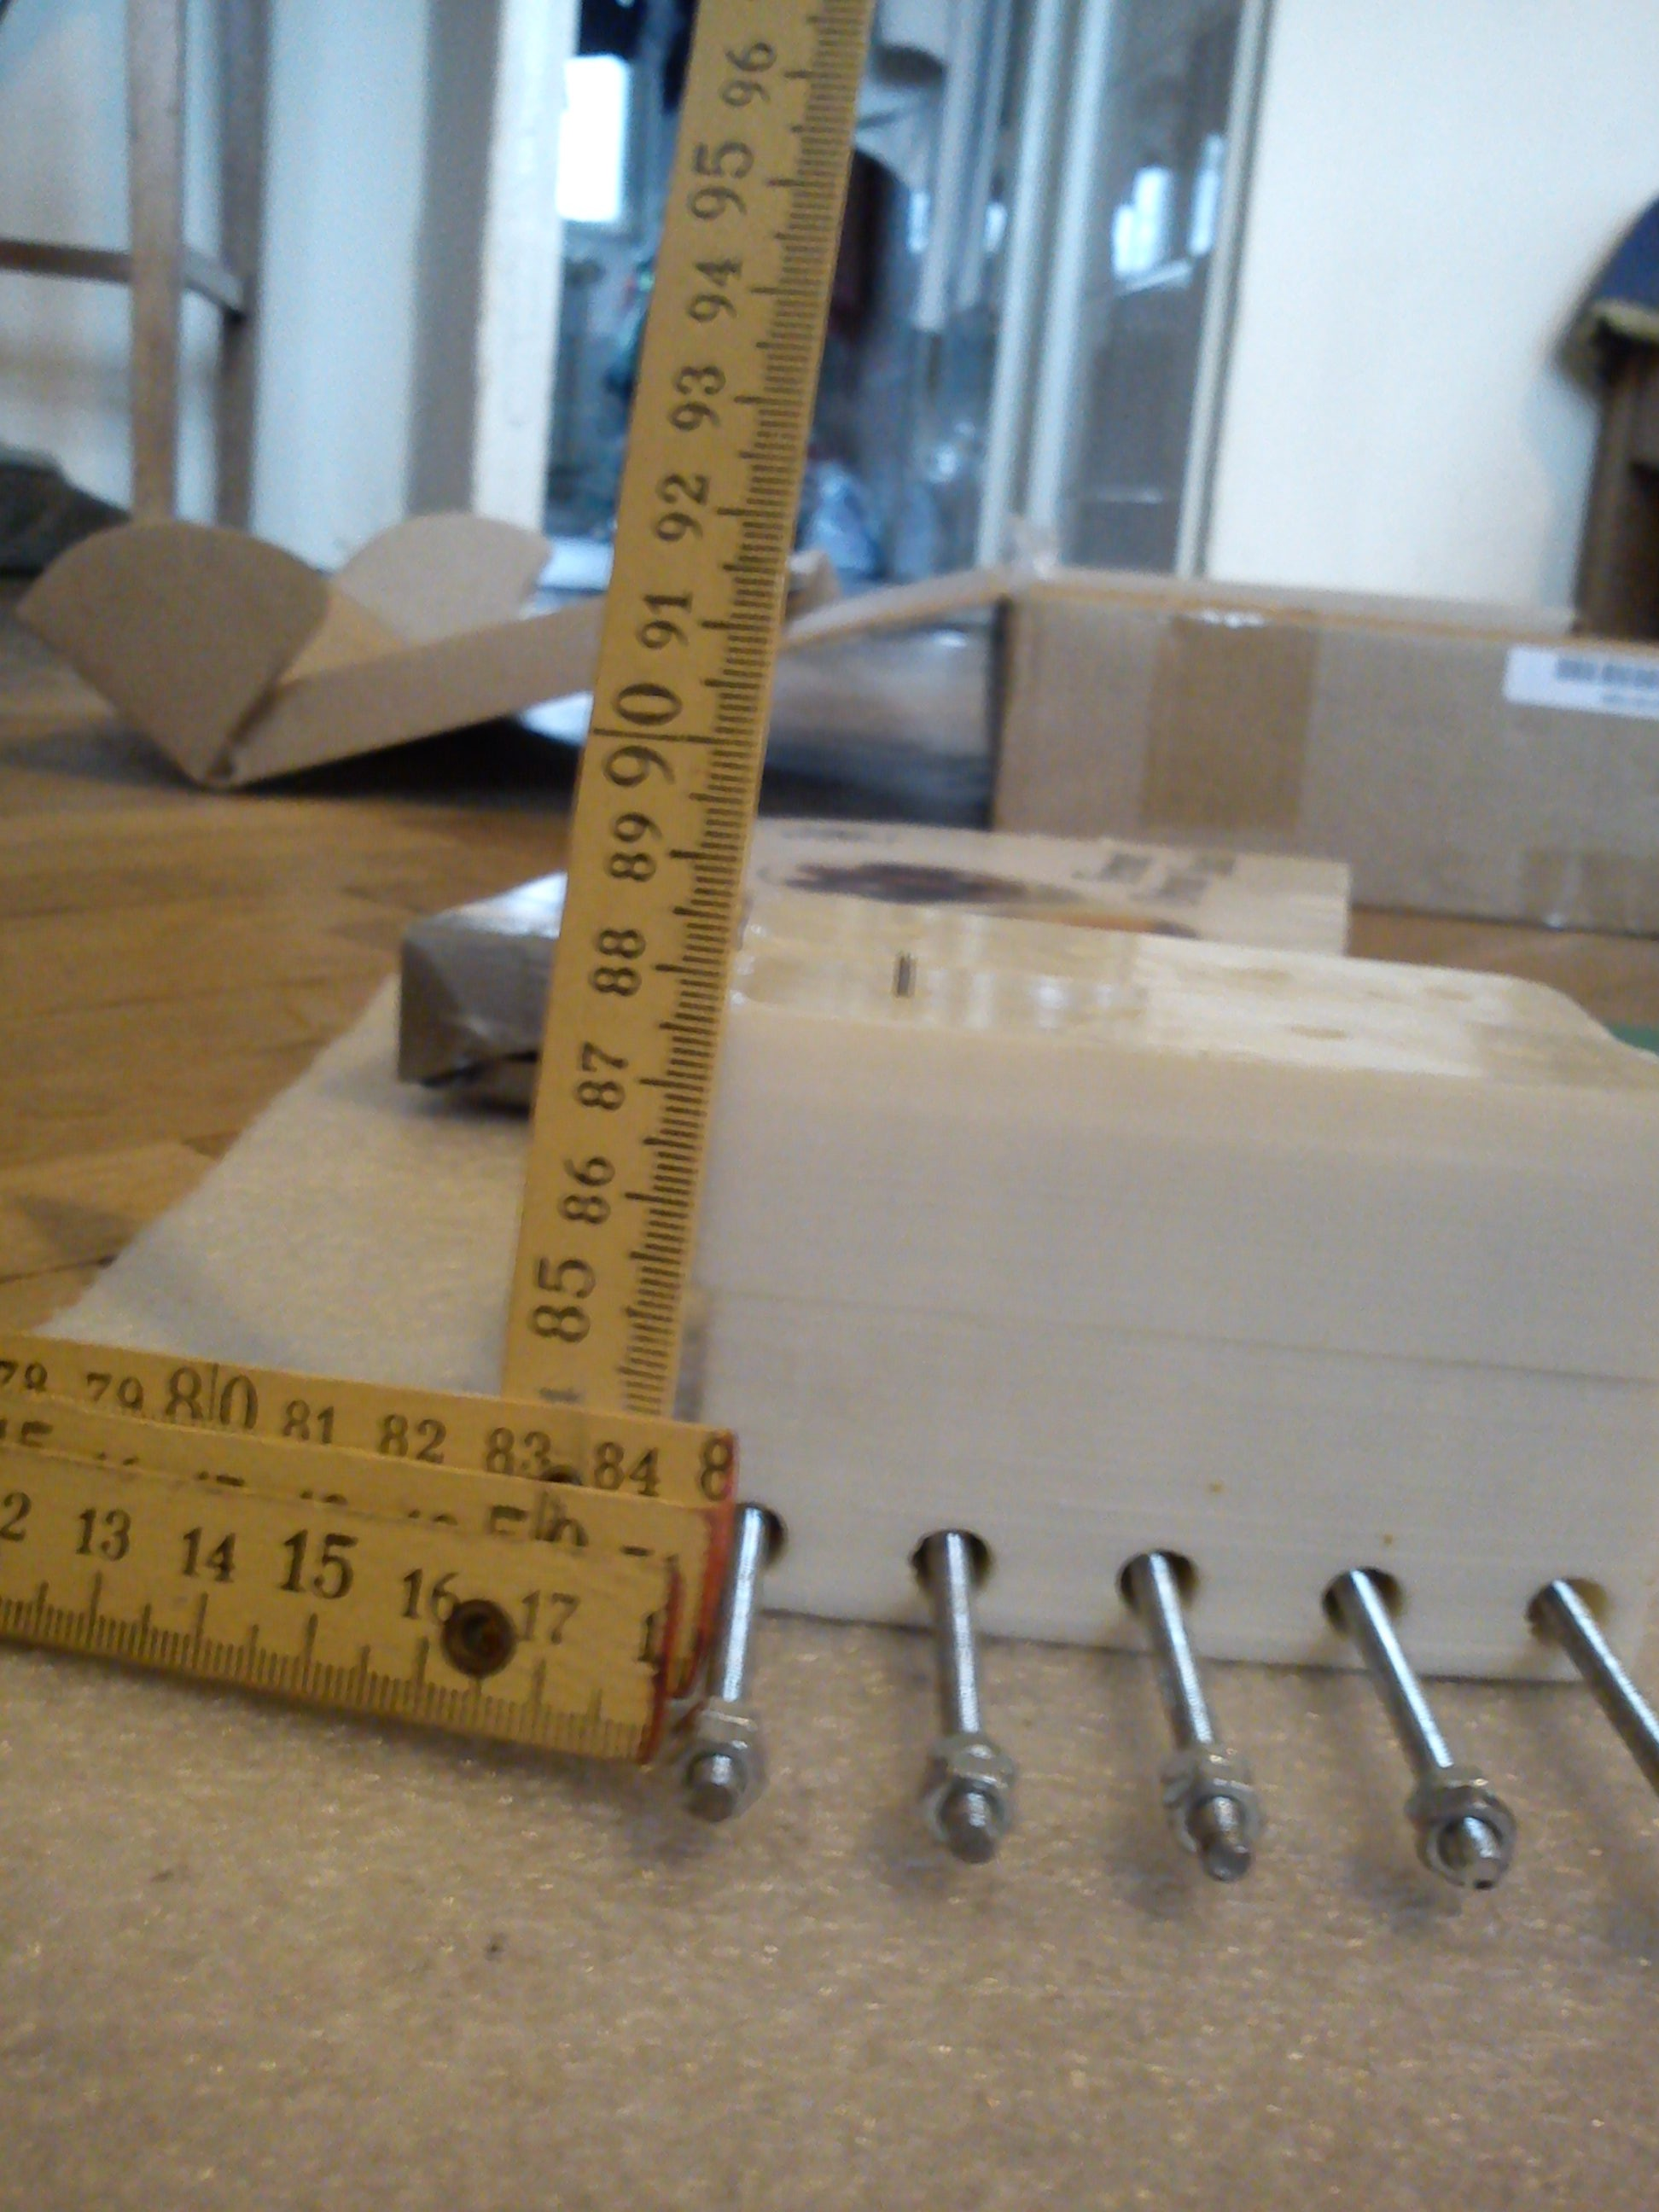
\includegraphics[width=.8\linewidth]{Device2}
  \caption{Obrazek 2 - Zobrazovač ze strany}
  \label{fig:sub1}
\end{subfigure}%
\begin{subfigure}{.5\textwidth}
  \centering
  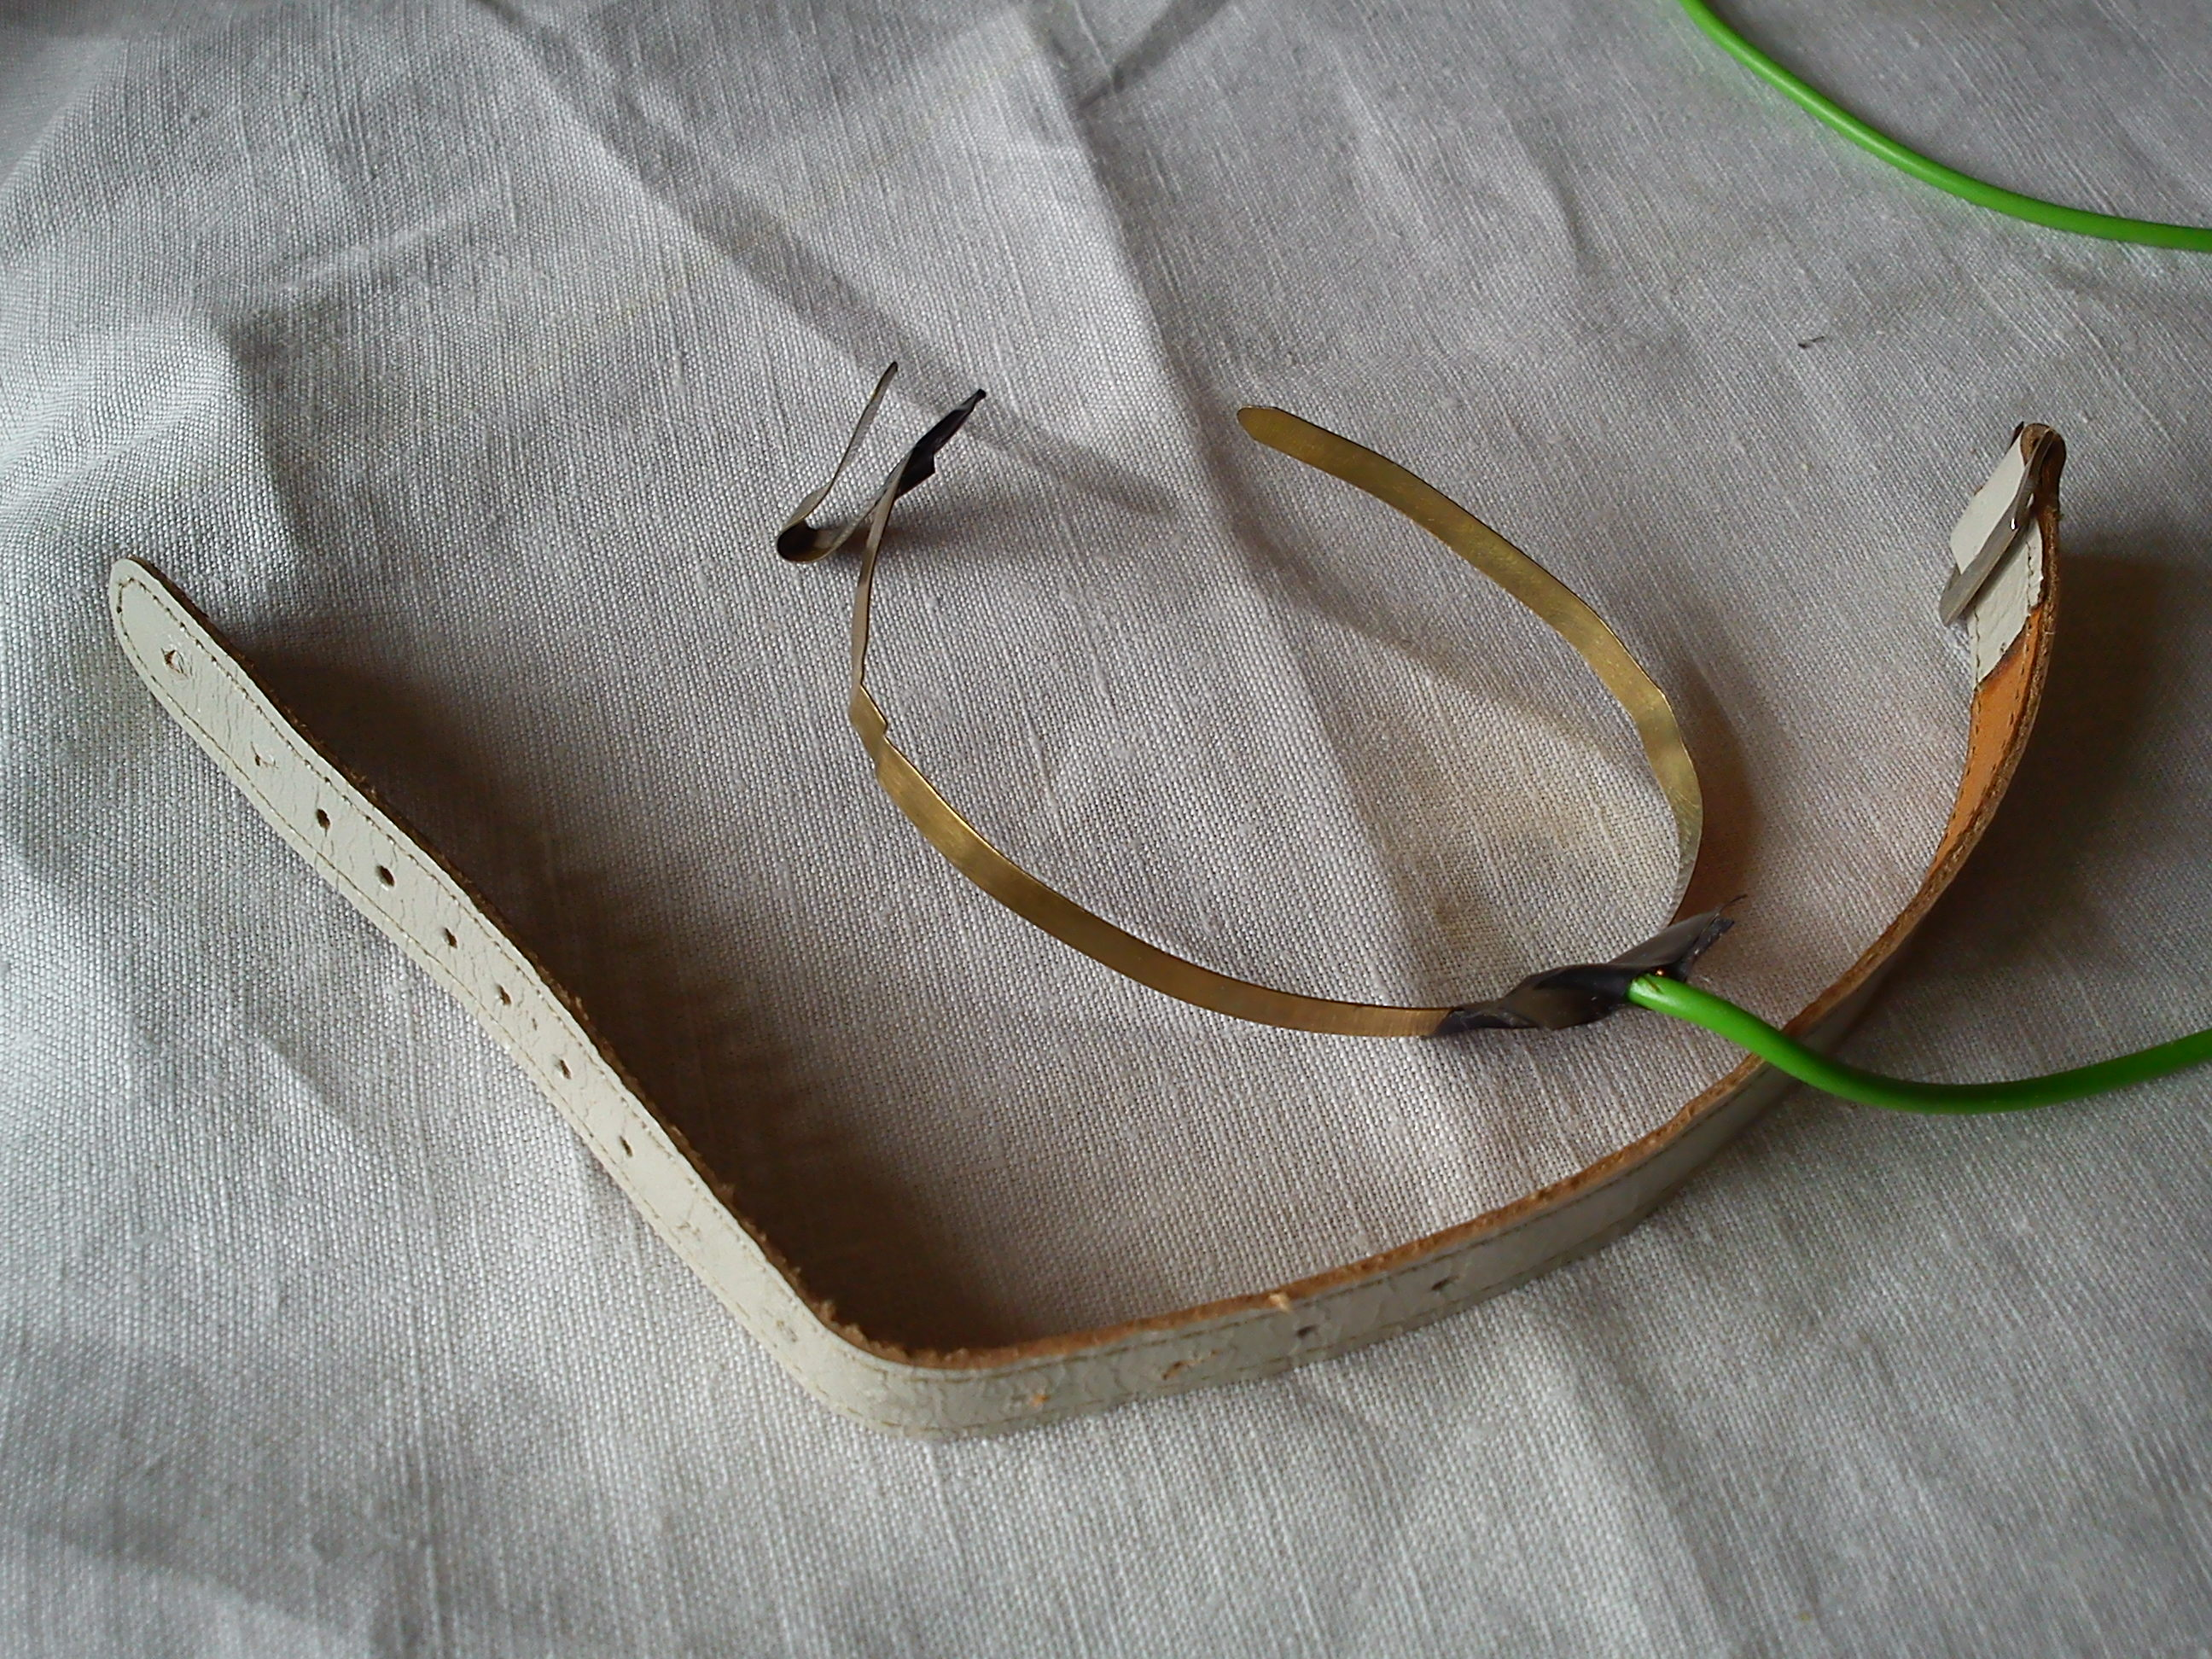
\includegraphics[width=.8\linewidth]{Device3}
  \caption{Obrazek 3 - Zapesní elektrod}
  \label{fig:sub2}
\end{subfigure}
\label{fig:test}
\end{figure}


\clearpage

\section{Texty}
\subsection{Tisknutý text}
\begin{verbatim}
Děkuji za Vaši účast v této
studii.
Vyzkoušíme nový braillský řádek!

V rámci této studie shromáždím ně-
jaká data o Vás a o tom, jak čtete
Braillovo písmo.  Tato data budou
při zveřejnění anonymní. Jedná se
o Váš přibližný věk, dosažené vzdě-
lání, zkušenost s Braillovým pís-
mem, audionahrávku našeho setkání a
záznam Vaší práce s nástrojem. Než
budeme pokračovat, potřebuji Váš
souhlas se shromážděním a zveřej-
něním těchto dat.

Následující text čtěte prosím na-
hlas a bez přestání až do konce.
Pokud budete mít nějaké otázky,
zeptejte se prosím až potom.

Začátek textu:
Dnes budete seznámen s novým druhem
braillského řádku, který se nazývá
FCHAD.  Tento řádek je navržen
s úmyslem vytvořit nejlevnější možný
                                   1

---- konec stranky ----
\end{verbatim}
\clearpage
\begin{verbatim}

zobrazovač vůbec. Zobrazuje text po
jednotlivých písmenech. Zobrazení
se ovládá pomocí řádku senzorů. Po-
ložením prstu na jeden z dvanácti
kovových bodíků vybíráte, které
z písmen v řádku chcete zobrazit.
Používáte obě ruce: jedna vybírá
písmeno, druhá ho čte.

Konec textu.

Teď Vám položím několik otázek
a poté vyzkoušíme nástroj.
 ---------------------
\end{verbatim}
% 138 + 4 capitals 262 + 3 captials
\clearpage
\subsection{Text na FCHAD}
\begin{multicols}{3}
\begin{verbatim}
Braills
ký řádek, kt
erý teď použ
íváte, není 
první řádek,
 který zobra
zuje jenom j
edno písmeno
.  První byl
 vynalezen v
 roce 1913 v
 Anglii.  Jm
enoval se Op
tofon a přev
áděl světlo 
na zvuk.  Kd
yž čtenář po
hyboval spec
iálním perem
 nad písmene
m, přístroj 
bzučel.  To 
bylo velmi p
omalé.  V še
desátých let
ech byl v Ka
lifornii vyn
alezen lepší
 nástroj.  T
akzvaný Opta
con převáděl
 světlo na v
ibrace a zob
razoval pomo
cí 144 drobn
ých tyček.  
To už bylo r
ychlejší, al
e přístroj b
yl hodně dra
hý.  FCHAD, 
který použív
áte právě te
ď, je dosud 
nejlevnější 
hmatový brai
llský zobraz
ovač.  Do bu
doucna by mo
hl být dostu
pný i v chud
ých zemích.
\end{verbatim}
\end{multicols}

